\documentclass[11pt,a4paper,]{article}
\usepackage{lmodern}

\usepackage{amssymb,amsmath}
\usepackage{ifxetex,ifluatex}
\usepackage{fixltx2e} % provides \textsubscript
\ifnum 0\ifxetex 1\fi\ifluatex 1\fi=0 % if pdftex
  \usepackage[T1]{fontenc}
  \usepackage[utf8]{inputenc}
\else % if luatex or xelatex
  \usepackage{unicode-math}
  \defaultfontfeatures{Ligatures=TeX,Scale=MatchLowercase}
\fi
% use upquote if available, for straight quotes in verbatim environments
\IfFileExists{upquote.sty}{\usepackage{upquote}}{}
% use microtype if available
\IfFileExists{microtype.sty}{%
\usepackage[]{microtype}
\UseMicrotypeSet[protrusion]{basicmath} % disable protrusion for tt fonts
}{}
\PassOptionsToPackage{hyphens}{url} % url is loaded by hyperref
\usepackage[unicode=true]{hyperref}
\hypersetup{
            pdfborder={0 0 0},
            breaklinks=true}
\urlstyle{same}  % don't use monospace font for urls
\usepackage{geometry}
\geometry{a4paper, centering, text={16cm,24cm}}
\usepackage[style=authoryear-comp,]{biblatex}
\addbibresource{references.bib}
\usepackage{longtable,booktabs}
% Fix footnotes in tables (requires footnote package)
\IfFileExists{footnote.sty}{\usepackage{footnote}\makesavenoteenv{long table}}{}
\usepackage{graphicx,grffile}
\makeatletter
\def\maxwidth{\ifdim\Gin@nat@width>\linewidth\linewidth\else\Gin@nat@width\fi}
\def\maxheight{\ifdim\Gin@nat@height>\textheight\textheight\else\Gin@nat@height\fi}
\makeatother
% Scale images if necessary, so that they will not overflow the page
% margins by default, and it is still possible to overwrite the defaults
% using explicit options in \includegraphics[width, height, ...]{}
\setkeys{Gin}{width=\maxwidth,height=\maxheight,keepaspectratio}
\IfFileExists{parskip.sty}{%
\usepackage{parskip}
}{% else
\setlength{\parindent}{0pt}
\setlength{\parskip}{6pt plus 2pt minus 1pt}
}
\setlength{\emergencystretch}{3em}  % prevent overfull lines
\providecommand{\tightlist}{%
  \setlength{\itemsep}{0pt}\setlength{\parskip}{0pt}}
\setcounter{secnumdepth}{5}

% set default figure placement to htbp
\makeatletter
\def\fps@figure{htbp}
\makeatother

% NEW:set default table placement to htbp
\makeatletter
\def\fps@table{htbp}
\makeatother


%% MONASH STUFF

%% CAPTIONS
\RequirePackage{caption}
\DeclareCaptionStyle{italic}[justification=centering]
 {labelfont={bf},textfont={it},labelsep=colon}
\captionsetup[figure]{style=italic,format=hang,singlelinecheck=true}
\captionsetup[table]{style=italic,format=hang,singlelinecheck=true}


%% FONT
\RequirePackage{bera}
\RequirePackage[charter,expert,sfscaled]{mathdesign}
\RequirePackage{fontawesome}

%% HEADERS AND FOOTERS
\RequirePackage{fancyhdr}
\pagestyle{fancy}
\rfoot{\Large\sffamily\raisebox{-0.1cm}{\textbf{\thepage}}}
\makeatletter
\lhead{\textsf{\expandafter{\@title}}}
\makeatother
\rhead{}
\cfoot{}
\setlength{\headheight}{15pt}
\renewcommand{\headrulewidth}{0.4pt}
\renewcommand{\footrulewidth}{0.4pt}
\fancypagestyle{plain}{%
\fancyhf{} % clear all header and footer fields
\fancyfoot[C]{\sffamily\thepage} % except the center
\renewcommand{\headrulewidth}{0pt}
\renewcommand{\footrulewidth}{0pt}}

%% MATHS
\RequirePackage{bm,amsmath}
\allowdisplaybreaks

%% GRAPHICS
\RequirePackage{graphicx}
\setcounter{topnumber}{2}
\setcounter{bottomnumber}{2}
\setcounter{totalnumber}{4}
\renewcommand{\topfraction}{0.85}
\renewcommand{\bottomfraction}{0.85}
\renewcommand{\textfraction}{0.15}
\renewcommand{\floatpagefraction}{0.8}


%\RequirePackage[section]{placeins}

%% SECTION TITLES


%% SECTION TITLES (NEW: Changing sections and subsections color)
\RequirePackage[compact,sf,bf]{titlesec}
\titleformat*{\section}{\Large\sf\bfseries\color[rgb]{0.8, 0.7, 0.1 }}
\titleformat*{\subsection}{\large\sf\bfseries\color[rgb]{0.8, 0.7, 0.1 }}
\titleformat*{\subsubsection}{\sf\bfseries\color[rgb]{0.8, 0.7, 0.1 }}
\titlespacing{\section}{0pt}{2ex}{.5ex}
\titlespacing{\subsection}{0pt}{1.5ex}{0ex}
\titlespacing{\subsubsection}{0pt}{.5ex}{0ex}


%% TITLE PAGE
\def\Date{\number\day}
\def\Month{\ifcase\month\or
 January\or February\or March\or April\or May\or June\or
 July\or August\or September\or October\or November\or December\fi}
\def\Year{\number\year}

%% LINE AND PAGE BREAKING
\sloppy
\clubpenalty = 10000
\widowpenalty = 10000
\brokenpenalty = 10000
\RequirePackage{microtype}

%% PARAGRAPH BREAKS
\setlength{\parskip}{1.4ex}
\setlength{\parindent}{0em}

%% HYPERLINKS
\RequirePackage{xcolor} % Needed for links
\definecolor{darkblue}{rgb}{0,0,.6}
\RequirePackage{url}

\makeatletter
\@ifpackageloaded{hyperref}{}{\RequirePackage{hyperref}}
\makeatother
\hypersetup{
     citecolor=0 0 0,
     breaklinks=true,
     bookmarksopen=true,
     bookmarksnumbered=true,
     linkcolor=darkblue,
     urlcolor=blue,
     citecolor=darkblue,
     colorlinks=true}

\usepackage[showonlyrefs]{mathtools}
\usepackage[no-weekday]{eukdate}

%% BIBLIOGRAPHY

\makeatletter
\@ifpackageloaded{biblatex}{}{\usepackage[style=authoryear-comp, backend=biber, natbib=true]{biblatex}}
\makeatother
\ExecuteBibliographyOptions{bibencoding=utf8,minnames=1,maxnames=3, maxbibnames=99,dashed=false,terseinits=true,giveninits=true,uniquename=false,uniquelist=false,doi=false, isbn=false,url=true,sortcites=false}

\DeclareFieldFormat{url}{\texttt{\url{#1}}}
\DeclareFieldFormat[article]{pages}{#1}
\DeclareFieldFormat[inproceedings]{pages}{\lowercase{pp.}#1}
\DeclareFieldFormat[incollection]{pages}{\lowercase{pp.}#1}
\DeclareFieldFormat[article]{volume}{\mkbibbold{#1}}
\DeclareFieldFormat[article]{number}{\mkbibparens{#1}}
\DeclareFieldFormat[article]{title}{\MakeCapital{#1}}
\DeclareFieldFormat[article]{url}{}
%\DeclareFieldFormat[book]{url}{}
%\DeclareFieldFormat[inbook]{url}{}
%\DeclareFieldFormat[incollection]{url}{}
%\DeclareFieldFormat[inproceedings]{url}{}
\DeclareFieldFormat[inproceedings]{title}{#1}
\DeclareFieldFormat{shorthandwidth}{#1}
%\DeclareFieldFormat{extrayear}{}
% No dot before number of articles
\usepackage{xpatch}
\xpatchbibmacro{volume+number+eid}{\setunit*{\adddot}}{}{}{}
% Remove In: for an article.
\renewbibmacro{in:}{%
  \ifentrytype{article}{}{%
  \printtext{\bibstring{in}\intitlepunct}}}

\AtEveryBibitem{\clearfield{month}}
\AtEveryCitekey{\clearfield{month}}

\makeatletter
\DeclareDelimFormat[cbx@textcite]{nameyeardelim}{\addspace}
\makeatother

\author{\sf\Large\textbf{ Di Cui}\\ {\sf\large Master of Business Analytics\\[0.5cm]} \sf\Large\textbf{ Guanru Chen}\\ {\sf\large Master of Business Analytics\\[0.5cm]} \sf\Large\textbf{ Yunzhi Chen}\\ {\sf\large Master of Business Analytics\\[0.5cm]}}

\date{\sf\Date~\Month~\Year}
\makeatletter
\lfoot{\sf Cui, Chen, Chen: \@date}
\makeatother


%%%% PAGE STYLE FOR FRONT PAGE OF REPORTS

\makeatletter
\def\organization#1{\gdef\@organization{#1}}
\def\telephone#1{\gdef\@telephone{#1}}
\def\email#1{\gdef\@email{#1}}
\makeatother
  \organization{}

  \def\name{TGIF \newline Di Cui \&\newline Guanru Chen \&\newline Yunzhi Chen}

  \telephone{(03) 9905 2478}

  \email{questions@company.com}                 %NEW: New email addresss

\def\webaddress{\url{http://company.com/stats/consulting/}} %NEW: URl
\def\abn{12 377 614 630}                                    % NEW: ABN
\def\logo{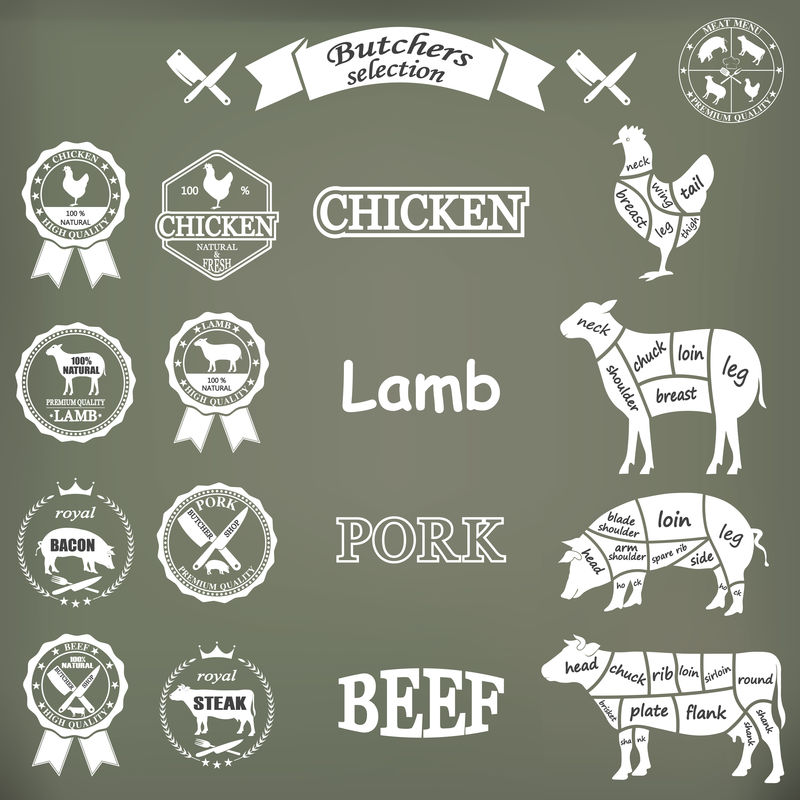
\includegraphics[width=6cm]{Figures/WeChat Image_20220521114617}}  %NEW: Changing logo
\def\extraspace{\vspace*{1.6cm}}
\makeatletter
\def\contactdetails{\faicon{phone} & \@telephone \\
                    \faicon{envelope} & \@email}
\makeatother

%%%% FRONT PAGE OF REPORTS

\def\reporttype{Report for}

\long\def\front#1#2#3{
\newpage
\begin{singlespacing}
\thispagestyle{empty}
\vspace*{-1.4cm}
\hspace*{-1.4cm}
\hbox to 16cm{
  \hbox to 6.5cm{\vbox to 14cm{\vbox to 25cm{
    \logo
    \vfill
    \parbox{6.3cm}{\raggedright
      \sf\color[rgb]{0.8, 0.7, 0.1 }    % NEW color 
      {\large\textbf{\name}}\par
      \vspace{.7cm}
      \tabcolsep=0.12cm\sf\small
      \begin{tabular}{@{}ll@{}}\contactdetails
      \end{tabular}
      \vspace*{0.3cm}\par
      ABN: \abn\par
    }
  }\vss}\hss}
  \hspace*{0.2cm}
  \hbox to 1cm{\vbox to 14cm{\rule{4pt}{26.8cm}\vss}\hss\hfill}  %NEW: Thicker line
  \hbox to 10cm{\vbox to 14cm{\vbox to 25cm{   
      \vspace*{3cm}\sf\raggedright
      \parbox{11cm}{\sf\raggedright\baselineskip=1.2cm
         \fontsize{24.88}{30}\color[rgb]{0, 0.29, 0.55}\sf\textbf{#1}}   % NEW: title color blue
      \par
      \vfill
      \large
      \vbox{\parskip=0.8cm #2}\par
      \vspace*{2cm}\par
      \reporttype\\[0.3cm]
      \hbox{#3}%\\[2cm]\
      \vspace*{1cm}
      {\large\sf\textbf{\Date~\Month~\Year}}
   }\vss}
  }}
\end{singlespacing}
\newpage
}

\makeatletter
\def\titlepage{\front{\expandafter{\@title}}{\@author}{\@organization}}
\makeatother

\usepackage{setspace}
\setstretch{1.5}

%% Any special functions or other packages can be loaded here.
\usepackage{booktabs}
\usepackage{longtable}
\usepackage{array}
\usepackage{multirow}
\usepackage{wrapfig}
\usepackage{float}
\usepackage{colortbl}
\usepackage{pdflscape}
\usepackage{tabu}
\usepackage{threeparttable}
\usepackage{threeparttablex}
\usepackage[normalem]{ulem}
\usepackage{makecell}
\usepackage{xcolor}


\begin{document}

\hypertarget{data-set-introduction}{%
\section{Data set introduction}\label{data-set-introduction}}

\hypertarget{research-questions}{%
\section{Research questions}\label{research-questions}}

\clearpage

\hypertarget{exploratory-data-analysis}{%
\section{Exploratory data analysis}\label{exploratory-data-analysis}}

<<<<<<< HEAD
<<<<<<< HEAD
\section*{}

\subsection*{Analysis}

\clearpage
=======
\clearpage

\section*{Per capita meat consumption}

\subsection*{Analysis}

\textbf{Which countries eat the most meat in the last 20 years? }

As can be seen from the Table \ref{tab:highest-meanconsumption} below, the top six countries with the highest average meat consumption mean in the world over the 20-year period from 1997 to 2017 are the United States, Australia, New Zealand, Spain, French Polynesia and Bahamas. The highest per capita meat consumption mean of the United States reached about 121.2 kg/capita/year. It can be concluded that countries with high income also consume more meat.
>>>>>>> Yunzhi_Chen

\section*{Brief about Meat Production}

<<<<<<< HEAD
\begin{itemize}
\item
  What's the production distribution of different livestock types across the world?
\item
  Which countries are main production country for?
\end{itemize}

\subsection*{Research Question}

\hypertarget{q1}{%
\subsection{Q1}\label{q1}}

\hypertarget{q1-1}{%
\subsection{Q1}\label{q1-1}}

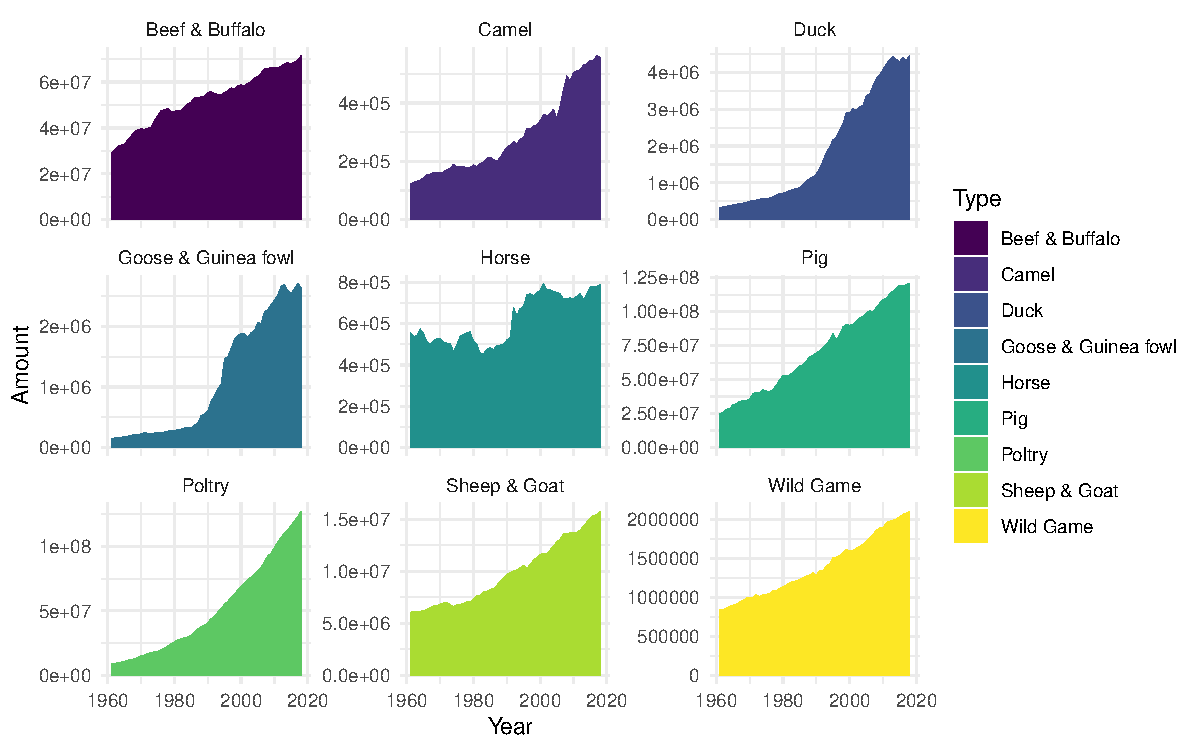
\includegraphics{report_files/figure-latex/productiontype-1.pdf} \includegraphics{report_files/figure-latex/productiontype-2.pdf}

In figure \ref{fig:fig1}, we see that the dominant livestock types are poultry, cattle (which includes beef and buffalo meat), pig, and sheep \& goat to a lesser extent at global level.

Although production of all major meat types have been increasing in absolute terms, in relative terms the share of global meat types have changed significantly over the last 50 years. In 1961, poultry meat accounted for small portion; by 2013 its share has tripled. In comparison, beef and buffalo meat as a share of total meat production has nearly halved. And the Pigmeat's share has remained more constant.

\clearpage

\hypertarget{q2}{%
\subsection{Q2}\label{q2}}

\begin{table}

\caption{\label{tab:cattle}Beef and buffalo (cattle) meat production, 1961-2018}
\centering
\begin{tabular}[t]{lr}
\toprule
Entity & Total\\
\midrule
World & 3048298992\\
Americas & 1355773399\\
Europe & 808420934\\
Northern America & 687736109\\
United States & 627725508\\
\addlinespace
South America & 568546284\\
Asia & 527122399\\
European Union & 494528637\\
Eastern Europe & 340150047\\
Low Income Food Deficit Countries & 296902586\\
\addlinespace
Net Food Importing Developing Countries & 291245656\\
Brazil & 289011599\\
Europe, Western & 243825958\\
Africa & 227535352\\
Southern Asia & 195483148\\
\addlinespace
USSR & 192970000\\
Eastern Asia & 192052963\\
Argentina & 155119322\\
China & 151848982\\
Least Developed Countries & 140568636\\
\bottomrule
\end{tabular}
\end{table}

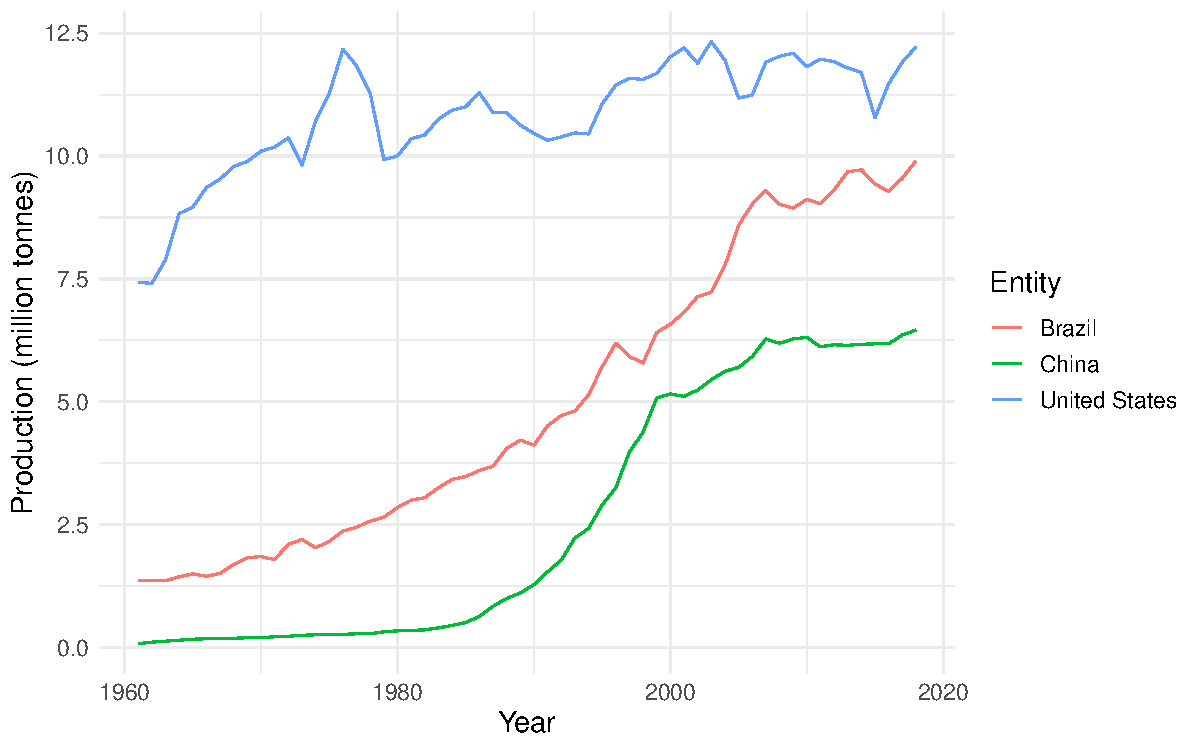
\includegraphics{report_files/figure-latex/cattle-1.pdf}

\begin{table}

\caption{\label{tab:poultry}Poultry meat production, 1961-2018}
\centering
\begin{tabular}[t]{lr}
\toprule
Entity & Total\\
\midrule
World & 3048298992\\
Americas & 1355773399\\
Europe & 808420934\\
Northern America & 687736109\\
United States & 627725508\\
\addlinespace
South America & 568546284\\
Asia & 527122399\\
European Union & 494528637\\
Eastern Europe & 340150047\\
Low Income Food Deficit Countries & 296902586\\
\addlinespace
Net Food Importing Developing Countries & 291245656\\
Brazil & 289011599\\
Europe, Western & 243825958\\
Africa & 227535352\\
Southern Asia & 195483148\\
\addlinespace
USSR & 192970000\\
Eastern Asia & 192052963\\
Argentina & 155119322\\
China & 151848982\\
Least Developed Countries & 140568636\\
\bottomrule
=======
\caption{\label{tab:highest-meanconsumption}Top 6 countries with the largest mean of meat consumption over years}
\centering
\begin{tabular}[t]{l|r}
\hline
Country & Mean\_consumption\_kg\_capita\_yr\\
\hline
United States & 121.19\\
\hline
Australia & 114.96\\
\hline
New Zealand & 105.19\\
\hline
Spain & 105.14\\
\hline
French Polynesia & 99.86\\
\hline
Bahamas & 98.57\\
\hline
>>>>>>> Yunzhi_Chen
\end{tabular}
\end{table}
\clearpage

<<<<<<< HEAD
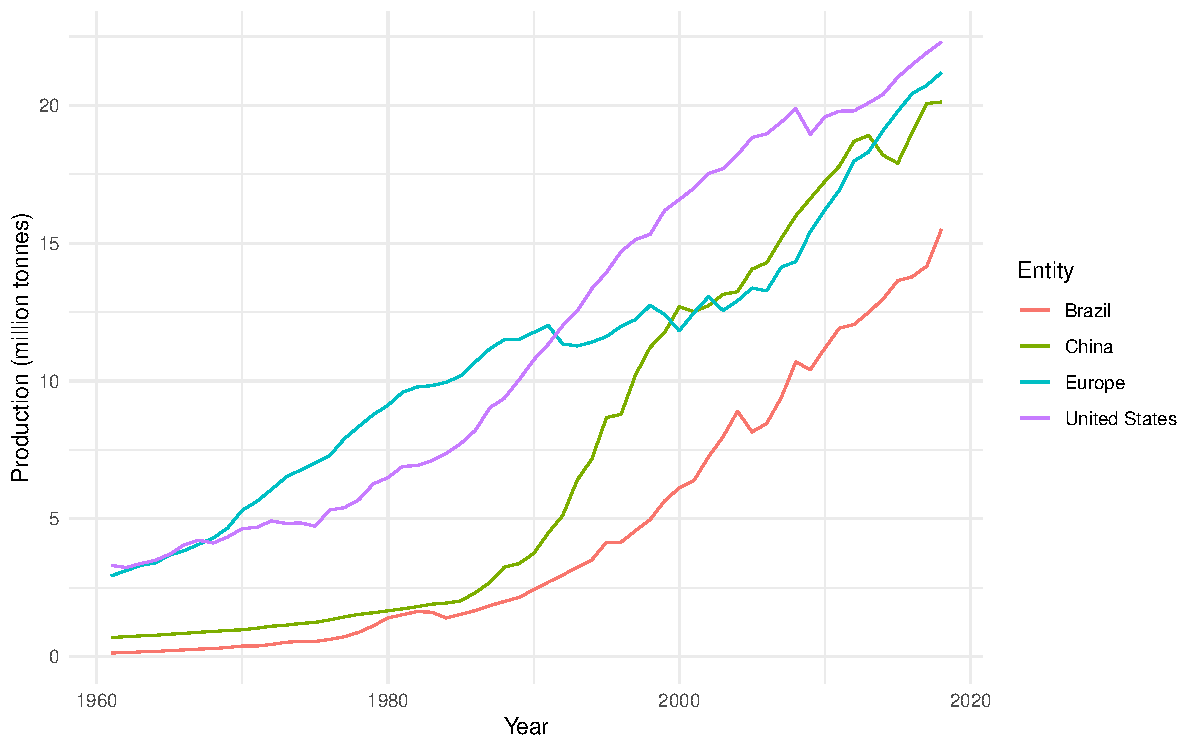
\includegraphics{report_files/figure-latex/poultry-1.pdf}

\begin{table}
=======
In terms of changing trends, figure \ref{fig:highest-consumption-trend} shows the meat consumption per person in these countries over the last 20 years have fluctuated considerably, with the exception of Australia and the United States, where consumption has increased, while all other countries have shown a decreasing trend, but the total value is still much higher than the world per capita meat consumption.
>>>>>>> Yunzhi_Chen

\caption{\label{tab:pig}Pig meat production, 1961-2018}
\centering
<<<<<<< HEAD
\begin{tabular}[t]{lr}
\toprule
Entity & Total\\
\midrule
World & 4097384349\\
Asia & 1898603248\\
Eastern Asia & 1669827471\\
China & 1560964337\\
Europe & 1381507340\\
\addlinespace
European Union & 1058781657\\
Americas & 757196334\\
Northern America & 523606187\\
Europe, Western & 506076170\\
Eastern Europe & 469050696\\
\addlinespace
United States & 450610222\\
Germany & 243524535\\
Southern Europe & 237607762\\
South Eastern Asia & 201427149\\
Northern Europe & 168772711\\
\addlinespace
South America & 161542187\\
USSR & 158895200\\
Low Income Food Deficit Countries & 122938347\\
Spain & 112057292\\
France & 107505681\\
\bottomrule
\end{tabular}
\end{table}

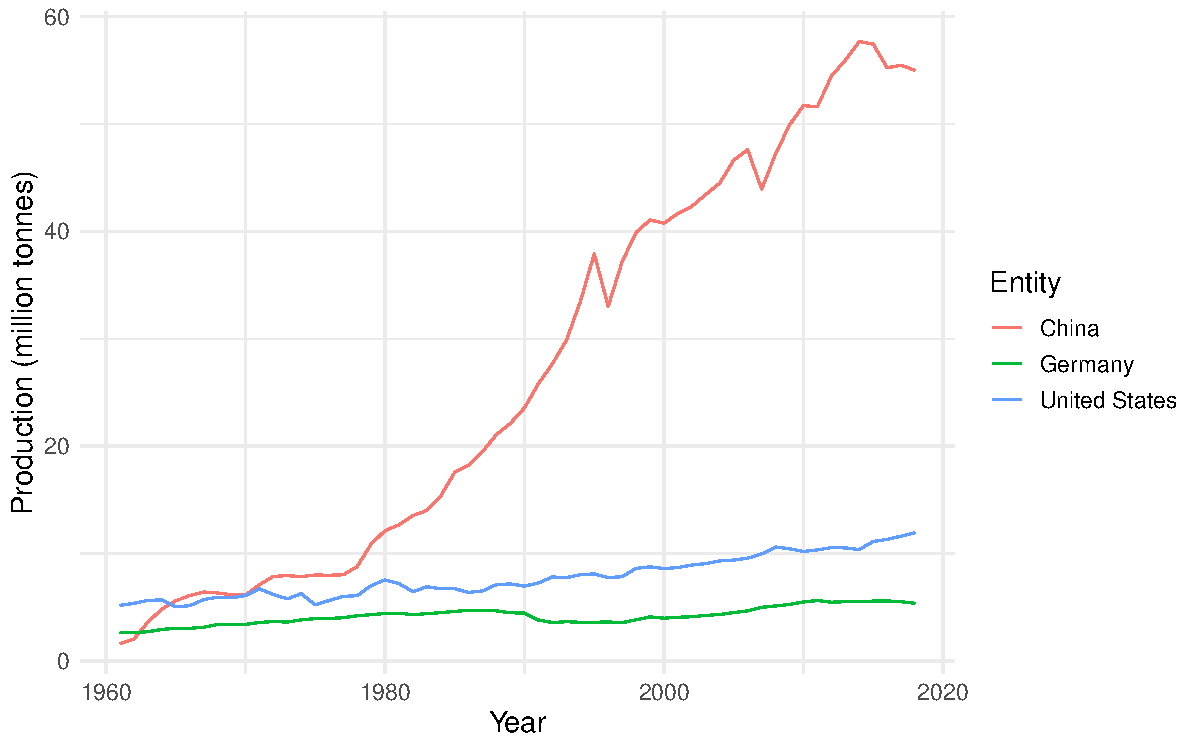
\includegraphics{report_files/figure-latex/pig-1.pdf}

In the table \ref{tab:cattle}, we see the global production of cattle (beef and buffalo) meat. From the country's perspective, The United States is the world's largest beef and buffalo meat producer. Other major producers are Brazil and China.

In the table \ref{tab:poultry}, we can see the production of poultry, like cattle production, the United States is still the world's largest producer. China and Brazil are also large poultry producers. Collectively, Europe is also a major poultry producer, just below the United States.

But for pigmeat production \ref{tab:pig}, China dominates global output, producing just short of half of total pigmeat. The other major producers include the United States, Germany.
\clearpage

\hypertarget{conclusion}{%
\section{Conclusion}\label{conclusion}}

=======
\section*{Global meat production -- Di Cui}

\subsection*{Analysis}

\textbf{Q1: How does global meat production develop from 1961 to 2018?}

\begin{figure}
\centering
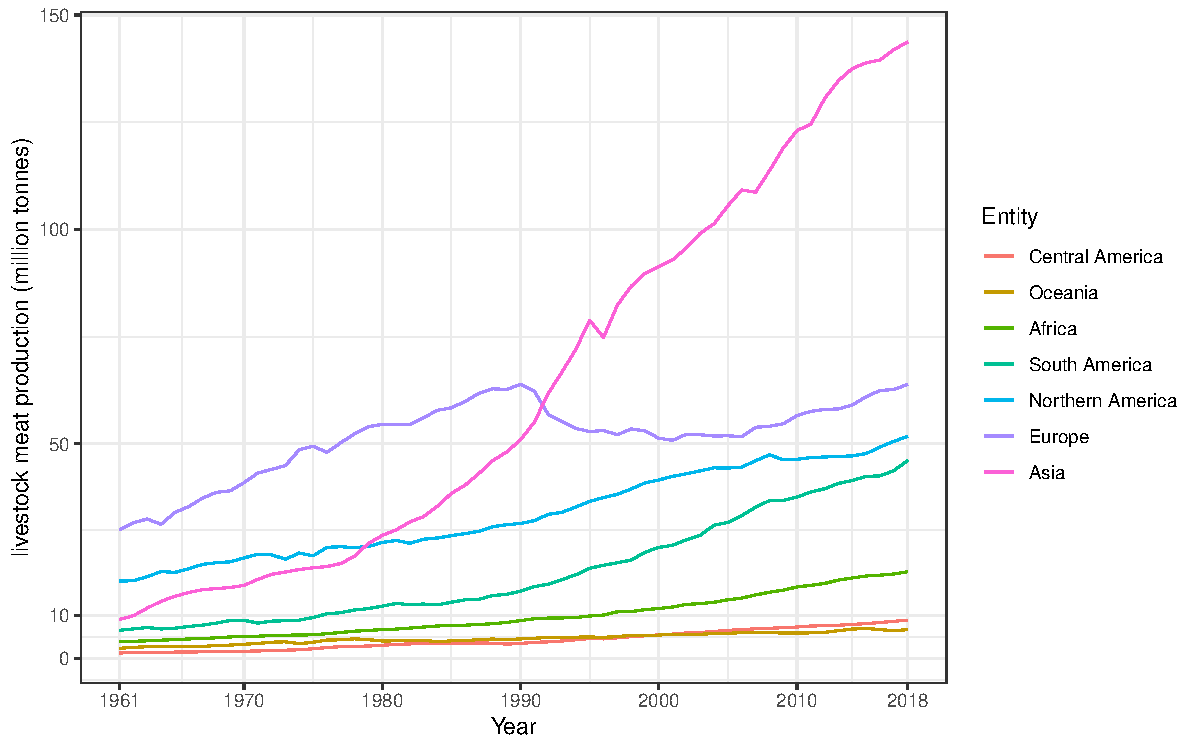
\includegraphics{report_files/figure-latex/continent-figure-1.pdf}
\caption{\label{fig:continent-figure}Global meat production from 1961 to 2018}
\end{figure}

From Figure\ref{fig:continent-figure}, we can see all continents show an uptrend. In particular, Asia production increased from under 10 million tonnes to around 150 million tonnes, and produced more meat than Europe in 1992, and become the largest meat production continent. And Europe shows a fluctuating growth, while another continents show steady growth.

\clearpage

\textbf{Q2: How do the Top six countries of meat production develop from 1961 to 2018?}

\begin{figure}
\centering
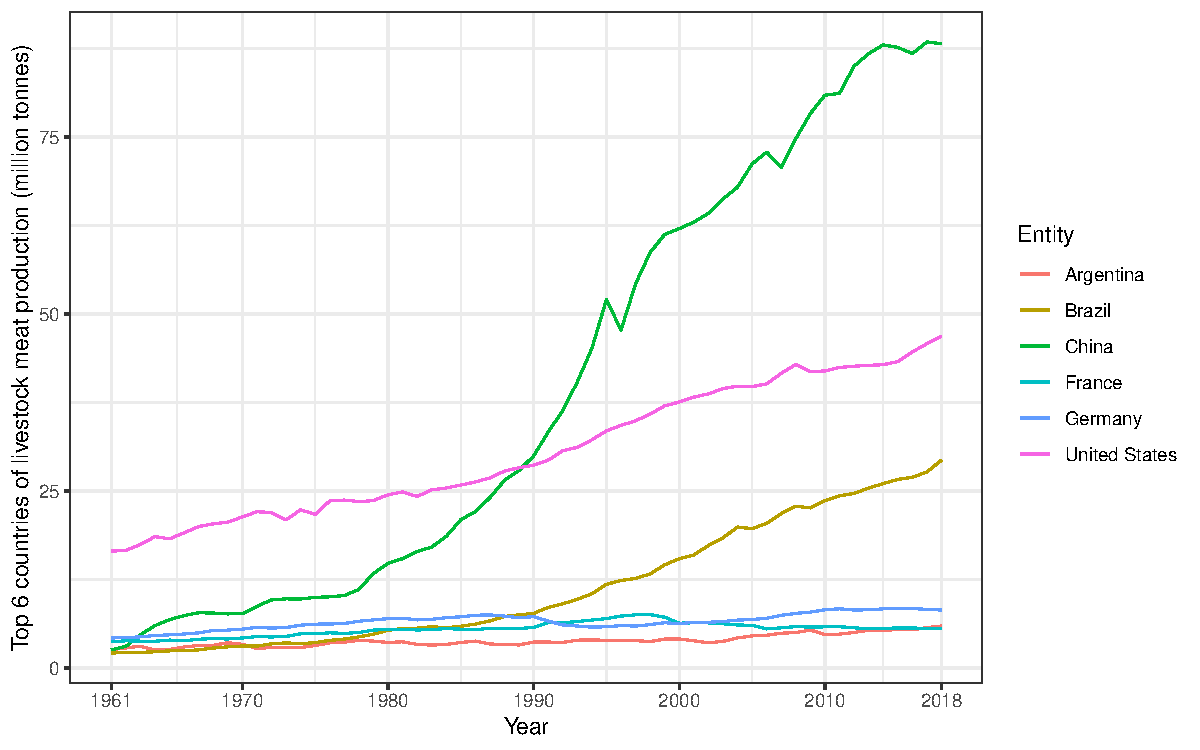
\includegraphics{report_files/figure-latex/country-1.pdf}
\caption{\label{fig:country}Top six countries' meat production from 1961 to 2018}
\end{figure}

From Figure\ref{fig:country}, it is obvious that China meat production has increased sharply. And China surpassed the United States in 1990 and became the largest meat production country in the world at the same time.

\clearpage

>>>>>>> 4f952e47aacfcce5877979dee0ef604f6632cda7
\section*{Citation}

The data set is cited from \textcite{meatproduction}.
=======
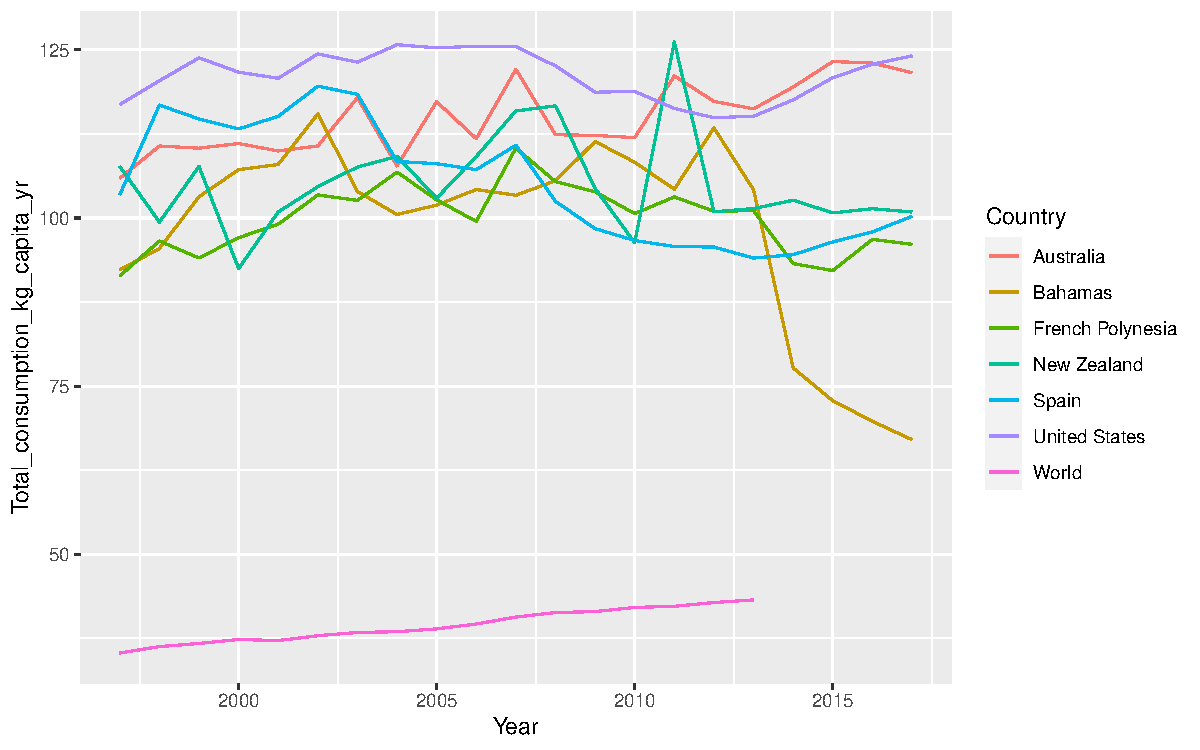
\includegraphics{report_files/figure-latex/highest-consumption-trend-1.pdf}
\caption{\label{fig:highest-consumption-trend}Consumption trend of top 6 countries}
\end{figure}

\clearpage

\textbf{What types of meat do people eat?}

From figure \ref{fig:Meat-type}, it illustrates that as a global average, pork has the highest per capita consumption of meat commodities; in 2013, per capita pork consumption was about 16 kg; followed by 15 kg of poultry; 9 kg of beef/buffalo meat; 2 kg of lamb and goat; and only a small percentage of other meats.

\begin{figure}
\centering
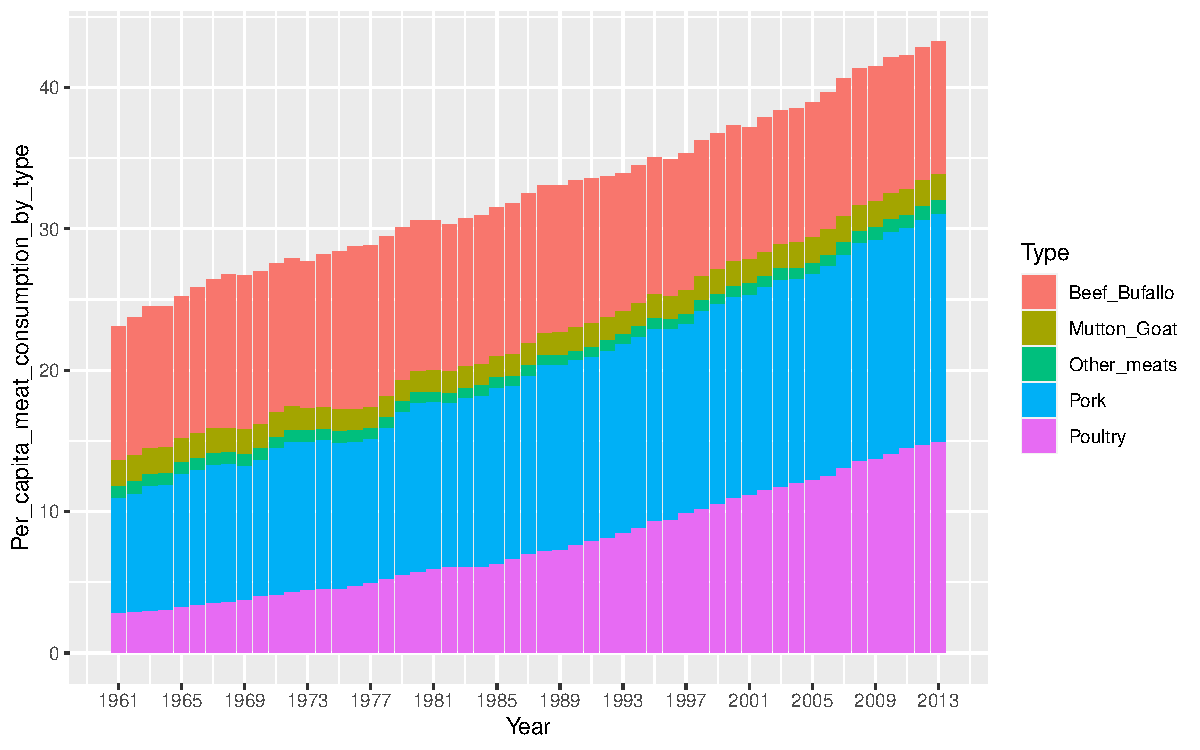
\includegraphics{report_files/figure-latex/Meat-type-1.pdf}
\caption{\label{fig:Meat-type}Meat type changes over time}
\end{figure}

\clearpage

\hypertarget{visualization-of-urbanization-energy-consumption-and-co2-emissions-with-different-income-level-countries}{%
\section{Visualization of urbanization, energy consumption, and CO2 emissions with different income level countries}\label{visualization-of-urbanization-energy-consumption-and-co2-emissions-with-different-income-level-countries}}

\hypertarget{conclusion}{%
\section{Conclusion}\label{conclusion}}

\section*{Citation}

The data set is cited from \textcite{owidmeatproduction}.
>>>>>>> Yunzhi_Chen

Analysis of the data is done using the following packages:

bookdown \textcite{bookdown1}, \textcite{bookdown2},

tidyverse \textcite{tidyverse},

readr \textcite{readr}

\printbibliography

\end{document}
